\documentclass[
	%a4paper, % Use A4 paper size
	letterpaper, % Use US letter paper size
]{jdf}

\addbibresource{references.bib}

\author{William Symon}
\email{wsymon3@gatech.edu}
\title{Project 1: Martingale - Final Report\\CS7646 - Fall 2025}

\begin{document}
%\lsstyle

\maketitle

\begin{abstract}
	In this report, we review the findings from the first project of the Fall 2025 semester of CS7646 - Machine Learning for Trading (ML4T). This project centered around writing code to simulate a given betting strategy on an American roulette wheel. The results of this simulation were then analyzed, allowing the student to gain a basic understanding of probability, risk, and statistical tools that will be utilized for the remainder of the course. An additional objective of this project was to familiarize the student with the course's workflow including the development environment, policies and standards, and submission process. 
\end{abstract}

\section{Introduction}
TODO: UPDATE TEXT

\section{Experiment 1}
TODO: UPDATE TEXT

\subsection{Setup}
TODO: UPDATE TEXT

\subsection{Data}
TODO: UPDATE TEXT

\subsection{Probability of Wining Exactly \$80 (Q1)}
TODO: UPDATE TEXT

\begin{jdffigure}
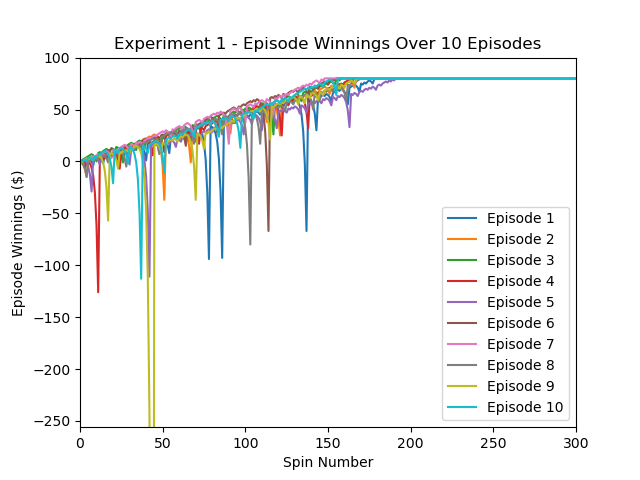
\includegraphics[height=9cm]{Figures/figure1.png}%
\captionof{figure}{Winnings per spin of 10 episodes for a bet of black on an American roulette wheel. Maximum winnings were capped at a value of \$80. }\label{fig:figure1}%
\end{jdffigure}

\subsubsection{Estimated Expected Value (Q2)}
TODO: UPDATE TEXT

\subsubsection{Exploration of Standard Deviation (Q3)}
TODO: UPDATE TEXT

\begin{jdffigure}
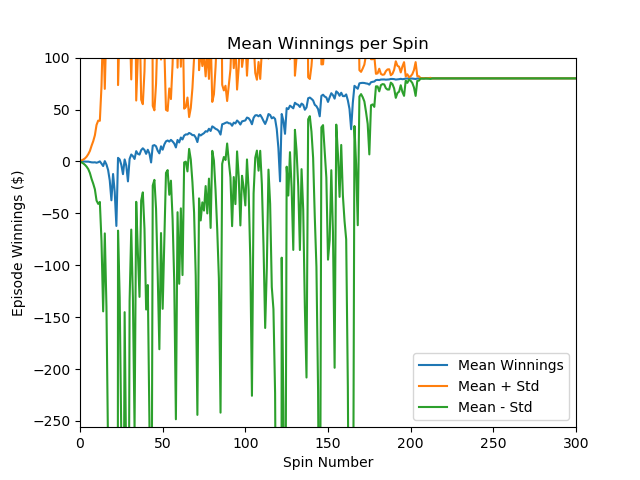
\includegraphics[height=9cm]{Figures/figure2.png}%
\captionof{figure}{Mean winnings over 1000 episodes per spin for a bet of black on an American roulette wheel. Maximum winnings were capped at a value of \$80. }\label{fig:figure2}%
\end{jdffigure}

\begin{jdffigure}
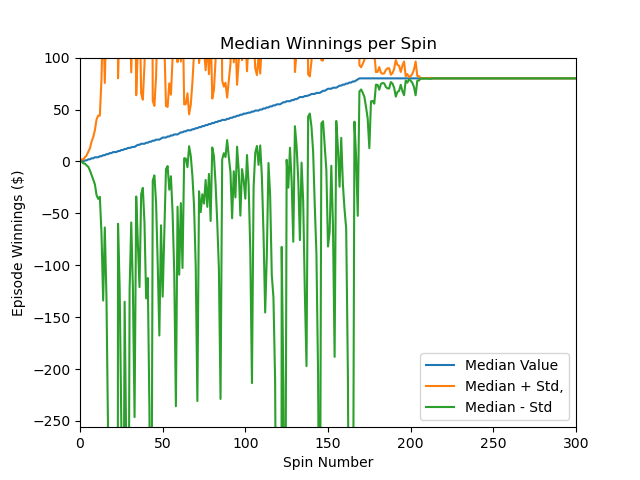
\includegraphics[height=9cm]{Figures/figure3.png}%
\captionof{figure}{Median winnings over 1000 episodes per spin for a bet of black on an American roulette wheel. Maximum winnings were capped at a value of \$80 }\label{fig:figure3}%
\end{jdffigure}

\section{Experiment 2}
TODO: UPDATE TEXT

\subsection{Setup}
TODO: UPDATE TEXT

\subsection{Data}
TODO: UPDATE TEXT

\subsection{Probability of Wining Exactly \$80 (Q4)}
TODO: UPDATE TEXT

\begin{jdffigure}
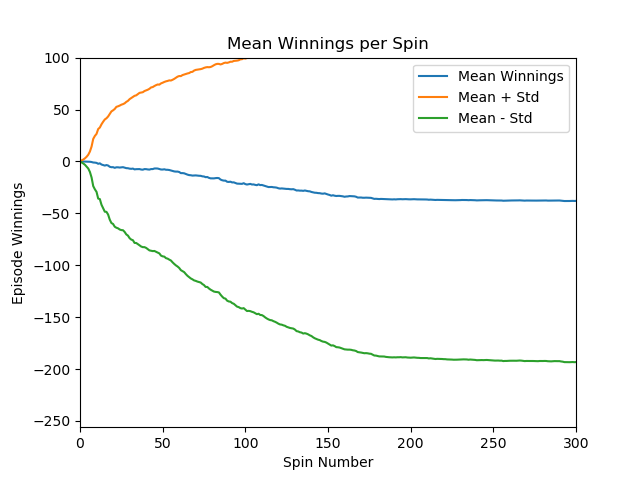
\includegraphics[height=9cm]{Figures/figure4.png}%
\captionof{figure}{Mean winnings over 1000 episodes per spin for a bet of black on an American roulette wheel. Maximum winnings were capped at a value of \$80. Minimum winnings were capped at -\$256 }\label{fig:figure4}%
\end{jdffigure}

\subsubsection{Estimated Expected Value (Q5)}
TODO: UPDATE TEXT

\subsubsection{Exploration of Standard Deviation (Q6)}
TODO: UPDATE TEXT

\begin{jdffigure}
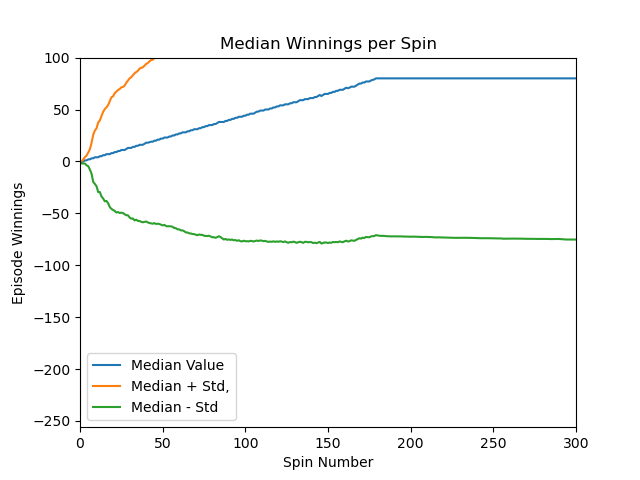
\includegraphics[height=9cm]{Figures/figure5.png}%
\captionof{figure}{Median winnings over 1000 episodes per spin for a bet of black on an American roulette wheel. Maximum winnings were capped at a value of \$80. Minimum winnings were capped at -\$256 }\label{fig:figure5}%
\end{jdffigure}

\section{Conclusion}
TODO: UPDATE TEXT

\subsection{Benefits of Expected Value (Q7)}
TODO: UPDATE TEXT

\subsection{Closing Thoughts}
TODO: UPDATE TEXT \citep{Martingale} \citep{Roulette}

\section{References}
\printbibliography[heading=none]

\end{document}
